\documentclass[10pt]{article}

%%%%%%%%%%%%%%%%%%%%%%%%%%%%%%%%%%%%%%%%%%%%%%%%%%%%%%%%%%%%%%%%%%%%%%%%%%%%%%%%%%%%%%%%%%%%%%%%%%%%%%%%%%%%%%%%%%%%%
%%                                              LOAD PACKAGES
%%%%%%%%%%%%%%%%%%%%%%%%%%%%%%%%%%%%%%%%%%%%%%%%%%%%%%%%%%%%%%%%%%%%%%%%%%%%%%%%%%%%%%%%%%%%%%%%%%%%%%%%%%%%%%%%%%%%%
\usepackage{ifpdf}
\usepackage[load-configurations=abbreviations]{siunitx}     % define units
\usepackage{color}                                          % add colors to text (and highlight)
\usepackage{soul}                                           % for highlighting
\usepackage{amsmath}                                        % for mathematical formula
\usepackage{amssymb}                                        % mathematical symbols (might not be useful)
\usepackage{booktabs}                                       % for arrays: toprule, midrule, bottomrule
\usepackage{multirow}                                       % for arrays
\usepackage{graphicx}                                       % for \includegraphics
\usepackage{rotating}                                       % for sideways and other rotating stuffs
\usepackage{authblk}                                        % for authors and affiliations
\usepackage[printonlyused,withpage]{acronym}
%\usepackage[printonlyused,withpage,nohyperlinks]{acronym}


\ifpdf
    \usepackage[subrefformat=parens]{subcaption}                % for subfigures (replaces the subfig package:
                                                                % more up-to-date and works well with hyperref)
    \pdfoptionpdfminorversion=6                                 % Solves "found PDF version 1.6, but at most version
                                                                % 1.5 allowed" warning
\fi

\usepackage[
            backend         = biber
            , style         = authoryear-comp   %numeric-comp, authoryear-comp
            , sorting       = nyt               % name, title, year
            , maxbibnames   = 10                % maximum number of authors to mention in the bibliography, if reached,
            , minbibnames   = 1                 % the number of authors to cite is set to minbibnames (et al.)
            , maxcitenames  = 2                 % same for within the text (makes sense with only specific cite styles)
            , mincitenames  = 1
            , backref       = false             % indicate or not the page on which the bibliography item is cited
            , backrefstyle  = three
            , abbreviate    = true              % default (Volume -> Vol., pages -> pp., ...)
            , doi           = false
            , isbn          = false
            , url           = false
            , eprint        = false
            , firstinits    = true              % all first and middle names as initials
            , uniquename    = init              % Disambiguate names using initials only (to be compatible with firstinits = true)
            ]{biblatex}

%\addbibresource{d:/KULeuven/PhD/MendeleyBiblioAbbr.bib}
%\addbibresource{d:/KULeuven/PhD/Publish/JournalPublications/Neuroimage/draft/AdditionalBiblioAbbr.bib}
\addbibresource{d:/KULeuven/PhD/MendeleyBiblio.bib}
%\addbibresource{d:/KULeuven/PhD/Publish/JournalPublications/Neuroimage/draft/AdditionalBiblio.bib}

% TO LOAD LAST FOR COMMANDS NOT TO BE OVERWRITTEN
\usepackage[bookmarksopen,colorlinks,linkcolor=blue,citecolor=blue]{hyperref} % for \autoref and hyperlinks

%%%%%%%%%%%%%%%%%%%%%%%%%%%%%%%%%%%%%%%%%%%%%%%%%%%%%%%%%%%%%%%%%%%%%%%%%%%%%%%%%%%%%%%%%%%%%%%%%%%%%%%%%%%%%%%%%%%%%
%%                                           DOCUMENT OPTIONS
%%%%%%%%%%%%%%%%%%%%%%%%%%%%%%%%%%%%%%%%%%%%%%%%%%%%%%%%%%%%%%%%%%%%%%%%%%%%%%%%%%%%%%%%%%%%%%%%%%%%%%%%%%%%%%%%%%%%%

%--------------------------------------------------
% biblatex options
%--------------------------------------------------

%% remove "in:" from articles
%\renewbibmacro*{in:}{%
%  \ifentrytype{article}{}{%
%    \printtext{%
%      \bibstring{in}\intitlepunct}}}

%\renewcommand{\newunitpunct}{}
%\renewcommand{\newblockpunct}{}

% remove "in" before journal/conference/... title
\renewbibmacro*{in:}{}

% remove "month" from all entries
\AtEveryBibitem{%
  \clearfield{month}%
}

% in bibliography: last name, first name
\DeclareNameAlias{sortname}{last-first}

% remove quote for title (remove italic for book title) (check original in biblatex.def)
\DeclareFieldFormat
  [article,inbook,incollection,inproceedings,patent,thesis,unpublished,book]
  {title}{#1\isdot}

% remove pp. for pages
\DeclareFieldFormat
  [article,inbook,incollection,inproceedings]
  {pages}{#1}

% remove italic for journal/collection/proceeding title
\DeclareFieldFormat{journaltitle}{#1}
\DeclareFieldFormat{booktitle}{{#1}}

% remove parenthesis from year
\makeatletter
\def\act@on@bibmacro#1#2{%
  \expandafter#1\csname abx@macro@\detokenize{#2}\endcsname
}
\def\patchbibmacro{\act@on@bibmacro\patchcmd}
\def\pretobibmacro{\act@on@bibmacro\pretocmd}
\def\apptobibmacro{\act@on@bibmacro\apptocmd}
\def\showbibmacro{\act@on@bibmacro\show}
\makeatother

\patchbibmacro{date+extrayear}{%
  \printtext[parens]%
}{%
  \addcomma\space%
  \printtext%
}{}{}

% volume (number) formatting
\newbibmacro*{volume+number+eid}{%
  \printfield{volume}%
  %\space%
  \iffieldundef{number}{}{
  \printtext[parens]{%
  \printfield{number}}%
  \setunit{\addcomma\space}%
  \printfield{eid}}}

% Citation Hyperlinks (not just years), thanks to Audrey.
\makeatletter
\renewbibmacro*{cite}{% Based on cite bib macro from authoryear-comp.cbx
  \iffieldundef{shorthand}
    {\ifthenelse{\ifnameundef{labelname}\OR\iffieldundef{labelyear}}
       {\printtext[bibhyperref]{% Include labelname in hyperlink
          \DeclareFieldAlias{bibhyperref}{default}% Prevent nested hyperlinks
          \usebibmacro{cite:label}%
          \setunit{\addspace}%
          \usebibmacro{cite:labelyear+extrayear}}%
          \usebibmacro{cite:reinit}}
       {\iffieldequals{namehash}{\cbx@lasthash}
          {\ifthenelse{\iffieldequals{labelyear}{\cbx@lastyear}\AND
                       \(\value{multicitecount}=0\OR\iffieldundef{postnote}\)}
             {\setunit{\addcomma}%
              \usebibmacro{cite:extrayear}}
             {\setunit{\compcitedelim}%
              \usebibmacro{cite:labelyear+extrayear}%
              \savefield{labelyear}{\cbx@lastyear}}}
          {\printtext[bibhyperref]{% Include labelname in hyperlink
             \DeclareFieldAlias{bibhyperref}{default}% Prevent nested hyperlinks
             \printnames{labelname}%
             \setunit{\nameyeardelim}%
             \usebibmacro{cite:labelyear+extrayear}}%
             \savefield{namehash}{\cbx@lasthash}%
             \savefield{labelyear}{\cbx@lastyear}}}}
    {\usebibmacro{cite:shorthand}%
     \usebibmacro{cite:reinit}}%
  \setunit{\multicitedelim}}

\renewbibmacro*{textcite}{% Based on textcite bib macro from authoryear-comp.cbx
  \iffieldequals{namehash}{\cbx@lasthash}
    {\iffieldundef{shorthand}
       {\ifthenelse{\iffieldequals{labelyear}{\cbx@lastyear}\AND
                    \(\value{multicitecount}=0\OR\iffieldundef{postnote}\)}
          {\setunit{\addcomma}%
           \usebibmacro{cite:extrayear}}
          {\setunit{\compcitedelim}%
           \usebibmacro{cite:labelyear+extrayear}%
           \savefield{labelyear}{\cbx@lastyear}}}
       {\setunit{\compcitedelim}%
        \usebibmacro{cite:shorthand}%
        \global\undef\cbx@lastyear}}
    {\ifnameundef{labelname}
       {\printtext[bibhyperref]{% Include labelname in hyperlink
          \DeclareFieldAlias{bibhyperref}{default}% Prevent nested hyperlinks
          \iffieldundef{shorthand}
            {\usebibmacro{cite:label}%
             \setunit{%
               \global\booltrue{cbx:parens}%
               \addspace\bibopenparen}%
             \ifnumequal{\value{citecount}}{1}
               {\usebibmacro{prenote}}
               {}%
             \usebibmacro{cite:labelyear+extrayear}}
            {\usebibmacro{cite:shorthand}}%
          \ifthenelse{\iffieldundef{postnote}\AND
                      \(\value{multicitetotal}=0\AND\value{citetotal}=1\)}
            {\bibcloseparen% Include closing parenthesis in hyperlink
             \global\boolfalse{cbx:parens}}
            {}}}
       {\printtext[bibhyperref]{% Include labelname in hyperlink
          \DeclareFieldAlias{bibhyperref}{default}% Prevent nested hyperlinks
          \printnames{labelname}%
          \setunit{%
            \global\booltrue{cbx:parens}%
            \addspace\bibopenparen}%
          \ifnumequal{\value{citecount}}{1}
            {\usebibmacro{prenote}}
            {}%
          \iffieldundef{shorthand}
            {\iffieldundef{labelyear}
               {\usebibmacro{cite:label}}
               {\usebibmacro{cite:labelyear+extrayear}}%
             \savefield{labelyear}{\cbx@lastyear}}
            {\usebibmacro{cite:shorthand}%
             \global\undef\cbx@lastyear}%
          \ifthenelse{\iffieldundef{postnote}\AND
                      \(\value{multicitetotal}=0\AND\value{citetotal}=1\)}
            {\bibcloseparen% Include closing parenthesis in hyperlink
             \global\boolfalse{cbx:parens}}
            {}}%
          \savefield{namehash}{\cbx@lasthash}}}%
  \setunit{%
    \ifbool{cbx:parens}
      {\bibcloseparen\global\boolfalse{cbx:parens}}
      {}%
    \multicitedelim}}

\makeatother



%--------------------------------------------------
% Define highlight color
%--------------------------------------------------
\definecolor{hlColor}{RGB}{255, 255, 102}
\sethlcolor{hlColor}

%--------------------------------------------------
% superscripts
%--------------------------------------------------
\newcommand{\superscript}[1]{\ensuremath{^{\textrm{#1}}}}
\newcommand{\nth}[0]{\superscript{th} }
\newcommand{\rd}[0]{\superscript{rd} }
%\newcommand{\st}[0]{\superscript{st}}

%--------------------------------------------------
% autoref names for hyperref package
%--------------------------------------------------
\def\figureautorefname{Fig.}
\def\sectionautorefname{sec.}
\def\subsectionautorefname{sec.}
\def\subsubsectionautorefname{sec.}
\def\equationautorefname{eq.}


%--------------------------------------------------
% line space: 1.3->1.5, 1.6->2
%--------------------------------------------------
%\linespread{1.6}

\ifpdf
    %--------------------------------------------------
    % page layout
    %--------------------------------------------------
    \addtolength{\topmargin}{-2cm}
    \addtolength{\textheight}{3cm}
    \addtolength{\evensidemargin}{-1.5cm}
    \addtolength{\oddsidemargin}{-1.5cm}
    \addtolength{\textwidth}{3cm}
\else
    %--------------------------------------------------
    %
    %--------------------------------------------------
    \makeatletter
    \newcommand\blx@unitmark{23sp}
    \makeatother
\fi



% fixes the issue with labels due to the acronym package
% http://tex.stackexchange.com/questions/109178/why-does-the-compiler-keeps-telling-me-forever-to-rerun-because-labels-have-ch
\makeatletter
\newcommand{\extraclearlabels}{\protected@write\@auxout{}{%
  \string\reset@newl@bel
}}
\makeatother

% define acronyms
\acrodef{SSVEP}{Steady-State Visually Evoked Potential}
\acrodef{BCI}{Brain-Computer Interface}
\acrodef{ERP}{Event Related Potential}
\acrodef{SVM}{Support Vector Machine}
\acrodef{EEG}{electroencephalography}
\acrodef{ERD}{Event Related Desynchronization}


%%%%%%%%%%%%%%%%%%%%%%%%%%%%%%%%%%%%%%%%%%%%%%%%%%%%%%%%%%%%%%%%%%%%%%%%%%%%%%%%%%%%%%%%%%%%%%%%%%%%%%%%%%%%%%%%%%%%%
%%%%%%%%%%%%%%%%%%%%%%%%%%%%%%%%%%%%%%%%%%%%%%%%%%%%%%%%%%%%%%%%%%%%%%%%%%%%%%%%%%%%%%%%%%%%%%%%%%%%%%%%%%%%%%%%%%%%%
%%%%%%%%%%%%%%%%%%%%%%%%%%%%%%%%%%%%%%%%%%%%%%%%%%%%%%%%%%%%%%%%%%%%%%%%%%%%%%%%%%%%%%%%%%%%%%%%%%%%%%%%%%%%%%%%%%%%%
%%%%%%%%%%%%%%%%%%%%%%%%%%%%%%%%%%%%%%%%%%%%%%%%%%%%%%%%%%%%%%%%%%%%%%%%%%%%%%%%%%%%%%%%%%%%%%%%%%%%%%%%%%%%%%%%%%%%%

\title{Hybrid oddball - SSVEP BCI}

\author[ * ]{A. Combaz, M. M. Van Hulle}
\affil[ * ]{Computational Neuroscience Group, Laboratory for Neuro- and Psychophysiology, KU Leuven, Leuven, Belgium}

\renewcommand\Authands{ and } % remove the comma before "and"

\begin{document}

%%%%%%%%%%%%%%%%%%%%%%%%%%%%%%%%%%%%%%%%%%%%%%%%%%%%%%%%%%%%%%%%%%%%%%%%%%%%%%%%%%%%%%%%%%%%%%%%%%%%%%%%%%%%%%%%%%%%%
%%                                           FRONTMATTER
%%%%%%%%%%%%%%%%%%%%%%%%%%%%%%%%%%%%%%%%%%%%%%%%%%%%%%%%%%%%%%%%%%%%%%%%%%%%%%%%%%%%%%%%%%%%%%%%%%%%%%%%%%%%%%%%%%%%%
\maketitle

\begin{abstract}
\extraclearlabels
Objectives:

Results:

Conclusion:
\end{abstract}

%%%%%%%%%%%%%%%%%%%%%%%%%%%%%%%%%%%%%%%%%%%%%%%%%%%%%%%%%%%%%%%%%%%%%%%%%%%%%%%%%%%%%%%%%%%%%%%%%%%%%%%%%%%%%%%%%%%%%
%%                                           MAIN TEXT
%%%%%%%%%%%%%%%%%%%%%%%%%%%%%%%%%%%%%%%%%%%%%%%%%%%%%%%%%%%%%%%%%%%%%%%%%%%%%%%%%%%%%%%%%%%%%%%%%%%%%%%%%%%%%%%%%%%%%

\acresetall

%===================================================================================================================
%                                             1 INTRODUCTION
%===================================================================================================================
\section{Introduction}
\label{sec:1Intro}

% General BCI
\acp{BCI} aim at decoding the brain activity in order to provide a direct communication channel between the brain and an external device.
In this study, the brain activity is recorded using \ac{EEG}, which offer the advantage over other method (\emph{e.g.} micro electrodes, fMRI \ldots) of being non-invasive and easy to set up.

% P3 BCI, definition, pluses and minuses
Some of the earliest \ac{EEG}-\ac{BCI} systems were based on the P3 component of the \ac{ERP} \parencite{Farwell1988, Donchin2000}.
The P3 is a positive deflection in the EEG time-locked to salient stimuli presented in an oddball paradigm, typically evoked over the parietal cortex, and occurs between \SIlist[list-units = single]{200;500}{\ms} after stimulus onset \parencite{Sutton1965}.
Although those \acp{BCI} rely mostly on the P3 component, other components (\emph{e.g.}, occipital N1 and/or N200) may also be used for ERP detection \parencite{Bianchi2010, Kaufmann2011}, for this reason we prefer here to use the term \emph{oddball-based \acp{BCI}}.
Such system have been shown to work successfully on both healthy and disabled subjects \parencite{Sellers2010, Krusienski2008, Combaz2013}.
However, as they rely on several repetition of a stimuli sequence in order to increase the signal-to-noise ratio of the \ac{ERP}, they remain slow and the communication speed decreases as the number of stimuli (\emph{i.e.} number of choices available to the user) increases.

% SSVEP BCI, definition, pluses and minuses
Other systems of interest are \acp{BCI} based on \acp{SSVEP}.
They rely on the psychophysiological properties of the EEG brain responses recorded from the occipital cortex during the periodic presentation of identical visual stimuli (\emph{i.e.} flickering stimuli).
When the periodic presentation is at a sufficiently high rate (\SI{>6}{\Hz}), stable and synchronized neural oscillations at the stimulus frequency and its harmonics are evoked over the visual cortex \parencite{Regan1966, Herrmann2001, Luck2005}.
Several \ac{SSVEP}-based \acp{BCI} have been successfully tested with healthy subjects (see \cite{Vialatte2010} for a review) and only recently (to a lesser extend) with locked-in patients \parencite{Parini2009, Combaz2013}.
Such \acp{BCI} have the advantage of a relatively fast detection, however, particularly when working with on-screen stimulation, the number of usable stimulation frequencies is limited \parencite{Bin2009}.
%on screen -> limited number of stimuli -> screen refresh rate, size of stimuli, distance between them and coamplification

% Hybrid BCI: definition
Recently, the \ac{BCI} community started to develop \emph{hybrid \acp{BCI}}, which combine different data acquisition modalities in order to improve the user experience of the system.
As defined by \textcite{Pfurtscheller2010}, \emph{``a typical hybrid \ac{BCI} is composed of one \ac{BCI} and another system (which might be another \ac{BCI}), and must also achieve specific goals better than a conventional system''}.
We focus here on the case where both system are \acp{BCI}.
The improvement achieved by a hybrid system can be of different natures such as higher accuracy, larger number of choice, higher selection speed, access to a no-control state, better usability or higher number of person effectively able to use the system \parencite{Brunner2011}.

% Hybrid BCI: same command for both system
A hybrid \ac{BCI} can be designed in a way that both modalities encode the same command, so that each of them could theoretically be used independently to make a decision.
Such system could help decreasing \ac{BCI} illiteracy (subject could compensate a weak control with one modality with a better control of the other) and/or increase the detection accuracy.
For example, \textcite{Allison2010a} showed in an offline analysis that \ac{ERD} and \ac{SSVEP} activity could be simultaneously elicited and detected and could lead to a wider number of people being able to control a two-choice \ac{BCI}.
They however observed in a later study analysing online data \parencite{Brunner2011}, that there was no significant difference between the pure \ac{SSVEP} and the hybrid condition.
An other example is the study from \textcite{Xu2013} where the authors combine detection of oddball response and detection of the interruption of \ac{SSVEP} response in a nine targets \ac{BCI} to improve the accuracy of the \ac{BCI}.

Other hybrid systems can be designed in a way that one modality can operate on its own while the other modality provides additional information helping to make the decision without being able to operate on its own.
This is the case of the study published by \textcite{Yin2013} where the authors use \ac{SSVEP} activity to increase the performance of an oddball-based spelling \ac{BCI}.

A last example of hybrid design is where each modality provides the system with independent commands that are then combined to result in a more complex control.
For example, \textcite{Allison2012} developed a \ac{BCI} where the user could control a cursor on a two dimensional screen where \ac{ERD} activity encoded vertical movement of the cursor and \ac{SSVEP} activity encoded horizontal movement.

To our knowledge, no design of such \emph{independent hybrid \ac{BCI}} combining the detection of \ac{SSVEP} activity and oddball \ac{ERP} has been reported on in the literature.
Neither has been proposed a study reporting on the influence of \ac{SSVEP} stimulation on the oddball response and the influence of visual oddball stimulation on \ac{SSVEP} responses with respect to the frequency used for the \ac{SSVEP} stimulation.
%This is what we propose in the present study.

We investigate the possibility to combine those two modalities in a way that would results in a system being able to operate faster than a purely oddball-based \ac{BCI} and encoding more targets than a purely \ac{SSVEP}-based \ac{BCI} would.
We aim here at studying the interactions between the two types of brain responses and the possibility of such a hybrid \ac{BCI} in a series of experiments where \ac{EEG} data are analysed offline.
This is a necessary first step before studying the differences in online performances between a hybrid system and purely oddball and \ac{SSVEP} based ones.

We report in this study on three series of experiment aiming at
1) studying the effect of a \ac{SSVEP} stimulation at different frequencies on the oddball response and its detection accuracy,
2) studying the effect of oddball stimulation on the \ac{SSVEP} response for different frequencies,
3) assessing the possibility to detect simultaneously both type of brain activity in a proof-of-concept experiment.






%% Hybrid BCI: general examples
%In their offline study, Allison showed that \ac{ERD} and \ac{SSVEP} activity could be simultaneously elicited and detected.
%Their results suggested that \ac{BCI} illiteracy could potentially be reduced by developing such system where one command could be detected by two different types of brain activity.
%In their online study (CITE), they showed that there was a significant improvement when comparing their hybrid \ac{BCI} to its pure \ac{ERD} counterpart in terms of performance and number of subjects who could effectively use the system, however there was no significant difference between the pure \ac{SSVEP} and the hybrid condition.
%
%This offline analysis suggested that such hybrid system could decrease \ac{BCI} illiteracy because subjects could compensate an eventual weak \ac{ERD} responses
%
%Offline analysis to show that ERD and SSVEP could be simultaneously elicited and detected and could potentially reduce BCI illiteracy
%Online implementation showed that

% Hybrid BCI: P3/SSVEP examples

% Hybrid BCI: what has not been done

% What we do here

%===================================================================================================================
%                                             2 MATERIALS AND METHODS
%===================================================================================================================
\section{Materials and Methods}
\label{sec:2MatAndMet}

    \subsection{Material}
    \label{sec:2.1Material}

    % EEG acq
    The EEG signals were recorded using a BioSemi Active Two system with 32~channels (following the 10-20 international system) at a sampling rate of \SI{1024}{\Hz}.
    Two additional electrodes were positioned on the right and left mastoids and the mean of the signals recorded at those two sites was used to reference the activity measured by the 32~EEG electrodes.

    % Stimuli presentation
    All stimulation employed MATLAB\textsuperscript{\textregistered}, the stimuli were visually presented on a laptop's LCD screen (\SI{60}{\Hz} refresh rate) and their display and timing used the \emph{Psychophysics Toolbox Extensions} \parencite{Brainard1997,Pelli1997}.

    The EEG data were processed using MATLAB\textsuperscript{\textregistered} and all statistical analyses were performed using R \parencite{R2013} and mixed effect models \parencite{Pinheiro2000} were fitted with the R package \emph{lme4} \parencite{lme42013}.


    \subsection{Experimental protocol}
    \label{sec:2.2Protocol}

        \subsubsection{Experiment 1: studying the oddball \acsp{ERP}}
        \label{sec:2.2.1ProtocolOddball}

        % Aim and subjects
        The aim of this first experiment was to study the effect of a flickering background on the typical \ac{ERP} response associated to an oddball paradigm.
        Nine subjects participated in the experiment (age, gender).

        % exp description
        As shown in \autoref{fig:stimSeq}, a typical \emph{stimulation cycle} (or \emph{trial}), started with a \SI{2000}{\ms} cue, indicating the participant his/her target item, followed by a \SI{1000}{\ms} pause during which the cue disappeared and all icons remained gray.
        The background rectangle started then to flicker and the oddball stimulation began \SI{500}{\ms} later.
        The oddball stimulation consisted of 10~\emph{flashing sequences} during which each of the 6~icons was flashed one after another in random order for a duration randomly set between \SIlist[list-units = single]{200;300}{\ms}.
        As usually done for oddball experiments, the participants were instructed to focus on their target symbol and count the number of time it flashes.
        A \SI{1000}{\ms} pause followed the oddball stimulation and preceded the next cue.
        An \emph{experimental run} lasted approximately 4~minutes and consisted of 12 consecutive trials, so that each of the 6~icons was cued twice (in random order).

        As we aimed here at studying the effect of the flickering background on the oddball \ac{ERP} response, we considered 5~experimental conditions.
        The first one (\emph{baseline condition}) consisted of a run as described in the previous paragraph but in which no flickering background was displayed.
        The 4~other conditions (\emph{hybrid conditions}) differed only by the frequency of the flickering background; the frequencies used were \SIlist[list-units = single]{8.57;10;12;15}{\Hz}, corresponding to the division of the refreshing rate of the screen by \numlist{7;6;5;4}, respectively.

        For each of the 5~conditions, all subjects performed 3~runs, therefore the whole experiment consisted of 15~runs of approximately 4~minutes each (12 trials per run).
        The order of the run was randomized for each subject and a 5~to~10~minutes pause was set up every 5~runs.

        % use
%        The data collected were used to compare the shape of the oddball response (response to the flashing of the target icon) and the \ac{ERP} classification accuracy (response to target \emph{v.s.} response to non-target flasing) across conditions.

        \subsubsection{Experiment 2: studying the \acs{SSVEP} responses}
        \label{sec:2.2.2ProtocolSSVEP}

        % Aim and subjects
        The aim of this second experiment was to study the effect of an oddball paradigm on the \ac{SSVEP} responses.
        N subjects participated in the experiment (age, gender).

        % exp description
        The experimental run was the same as described in \autoref{sec:2.2.1ProtocolOddball}.
        Two experimental parameters were manipulated, the first one was the stimulation frequency; the same frequencies as for the first experiment were used (\SIlist[list-units = single]{8.57;10;12;15}{\Hz}).
        The second experimental parameter was the presence or not of the oddball stimulation sequence.
        When the oddball stimulation was displayed, the participants were instructed to count the number of flashes of the target icon, while when no oddball stimulation was displayed, their task was simply to focus on their target icon.

        The experiment consisted thus of 8~runs of approximately 4~minutes each (12 trials per run).
        The order of the run was randomized for each subject and a 5~to~10~minutes pause was set up after the first 4~runs.

        % use
%        This experimental design allows a comparison of the \ac{SSVEP} responses of the participants with and without an oddball stimulation superimposed on the \ac{SSVEP} stimulation for a different set of \ac{SSVEP} frequencies.

        \subsubsection{Experiment 3: hybrid classification}
        \label{sec:2.2.3ProtocolHybrid}

%        After studying individually oddball \acp{ERP} and \ac{SSVEP} responses, we aim here at studying the possibility to detect both responses
        This third experiment consists in a proof-of-concept for a hybrid oddball-\ac{SSVEP} \ac{BCI}.
        N subjects took part in the experiment.

        Two rectangles flickering at \SI{12}{\Hz} and \SI{15}{\Hz} where simultaneously presented on the left and right side of the screen, respectively.
        Within each of those rectangles 6~items were presented so that 2~independent and simultaneous oddball paradigm could occur as shown in \autoref{fig:stim2oddball}.
        The \emph{stimulation cycle} was the same as described in \autoref{sec:2.2.1ProtocolOddball}, icons from the left and right rectangles were always flashed simultaneously, however the order in which the icons would be flashed was set independently (and randomly) for each rectangle.
        An \emph{experimental run} lasted approximately 4~minutes and consisted of 12 consecutive trials (with 10~repetitions of the flashing sequence for each), so that each of the 12~icons was cued once (in random order).
        Each subject participated in 8~consecutive runs with a 5~to 10~minutes pause after the the 4\nth run.


    \subsection{Data Analysis}
    \label{sec:2.3DataAnalysis}

        \subsubsection{Experiment 1: Observing the \acsp{ERP}}
        \label{sec:2.3.1AnalysisExp1}

        % observe ERP responses
        We first observed average responses to target stimuli for each of the 5~experimental conditions.
        The \ac{EEG} signals were filtered between \SIlist[list-units = single]{0.3;30}{\Hz} (zero-phase 3\rd order Butterworth filter) and epochs were cut from \SI{200}{\ms} before the stimuli onsets until \SI{800}{\ms} after.
        In order to ensure that none of the epochs used for averaging were corrupted by ocular artifact, we rejected, for each \emph{experimental run}, the 15\% epochs with the highest peak-to-peak amplitude \parencite{Luck2005}.
        We also visually inspected the filtered \ac{EEG} traces to verify that no of ocular artifact could be seen within the 85\% remaining epochs.
        For each participant, averaged \acp{ERP} were observed and compared with respect to the experimental condition.
        We particularly looked for differences between the baseline condition (pure oddball) and the hybrid conditions (4 other condition with flickering square) %and within the hybrid conditions themselves for an eventual influence of the flickering frequency over the \ac{ERP} response.

        To assess differences and similarities, we calculated for each subject and EEG channel the correlation coefficient between average ERPs for all \emph{conditions pairs} (5~experimental condition, 10~condition pairs, \emph{e.g.} oddball/hybrid-10Hz, hybrid-12Hz/hybrid-10Hz, \emph{etc}).
        Those correlation data were modelled with a linear-mixed effect model with the channels nested within subjects as a random effect and the condition pair as a fixed effect.
        Post-hoc pairwise comparisons for each level of the \emph{conditions pair} factor were conducted via Tukey's test (using the \emph{multcomp} R package, \cite{multcomp2008}).
        %The p-values obtained from the model were obtained via Markov-chain Monte Carlo (MCMC) sampling \parencite{Baayen2008}.
        The significance level was $\alpha = 0.01$.

        \subsubsection{Experiment 1: Classifying the \acsp{ERP}}
        \label{sec:2.3.1AnalysisExp1bis}

        % classify the ERPs
        The second step was to compare classification accuracies.
        The \ac{EEG} signals were filtered between \SIlist[list-units = single]{0.5;20}{\Hz} (zero-phase 3\rd order Butterworth filter), epochs were cut from each the stimuli onsets until \SI{600}{\ms} after and downsampled to \SI{128}{\Hz}.
        The resulting epochs were labeled to either \emph{target epochs} or \emph{non-target epochs} according to whether they corresponded to the \ac{EEG} response to a target stimulus (flashing of a target symbol) or a non-target one (flashing of any non-target symbol).
        For each subject and experimental condition, we ran a 3-fold cross-validation where a linear \ac{SVM} was trained \parencite{Keerthi2006} on the data collected during 2~out of the 3~experimental runs and the performance was measured on every trials of the remaining run.

        For each trial, the \ac{SVM} returns a score associated with each of the 6~icons and the icon with the highest score is identified as \emph{detected target}.
        We then derive a \emph{correctness value} set to 1~if the detected target matches the cued icon (correct detection) and 0~otherwise.
        We thus obtain for each subject and experimental condition 36~correctness values.
        The correctness values were computed for a number of repetitions $N_r$ of the flashing sequence varying from 1~to 10.
        In order to mimic the behavior of a \ac{BCI}, for each trial and each icon, epochs were average over the \emph{$N_r$ first repetitions}.

        % statistical model
        %The correctness data were analysed using R (\hl{CITE}) and the R package \emph{lme4} (\hl{CITE + languageR?}).
        The correctness data were modelled using a logistic mixed effect models \parencite{Jaeger2008a} with the number of repetitions nested within subjects as random factors.
        As fixed effects, we considered the experimental condition (5~levels factor), the number of repetitions (10~levels factor) and the interaction between those 2~factors.
        In order to assess of the influence of the experimental condition on the classification correctness we compared this model to a reduced version of it where the experimental condition factor (and all interactions involving this factor) was removed from the fixed effects.
        Both models were fitted using the \emph{maximum likelihood} method and the p-value was obtained by a \emph{likelihood ratio test} of the 2~models \parencite{Pinheiro2000}.

        \subsubsection{Experiment 1: single \emph{v.s.} multiple oddball classifier(s)}
        \label{sec:2.3.1AnalysisExp1ter}
        In the previous section, we measure performances by building one classifier for each subject and condition.
        More specifically, for each hybrid condition (\SIlist[list-units = single]{8.57;10;12;15}{\Hz}), a specific oddball ERP classifier is trained.
        In a hybrid oddball-SSVEP BCI, where several visual oddball paradigms occur simultaneously within SSVEP stimuli flickering at different frequencies, it does not seem convenient to have as many ERP classifiers as stimulation frequencies.
        First it would compromise the usability of the BCI by increasing the time needed for training, and second, as the target frequency is not known (this is the role of the SSVEP classifier to find it out), one would have to either rely on the SSVEP classifier to decide which ERP classifier to apply or to find an optimal design that combines the different ERP (and eventually SSVEP) classifiers in order to identify the target ERP.

        Ideally, it would be more appropriate to have a single ERP classifier trained on data recorded in all conditions.
        However this should not be done at the expense of a loss in detection accuracy.
        We thus compared accuracies of oddball ERP detection for data recorded in the hybrid condition obtained from classifiers built individually for each condition (as described in the previous section) to the accuracies resulting from a single classifier trained on all data recorded in the different hybrid conditions.

        As in the previous section, we modelled the correctness data using a logistic mixed effect models \parencite{Jaeger2008a} with the number of repetitions nested within subjects as random factors.
        As fixed effects, we considered the experimental condition (4~levels factor), the number of repetitions (10~levels factor), the type of classifier (2~levels factor) and all interactions between those 3~factors.
        In order to assess of the influence of the classifier on the classification correctness we compared this model to a reduced version of it where the classifier factor (and all interactions involving this factor) was removed from the fixed effects.
        Both models were fitted using the \emph{maximum likelihood} method and the p-value was obtained by a \emph{likelihood ratio test} of the 2~models \parencite{Pinheiro2000}.

%        We want therefore to compare the accuracies resulting from the classifiers build individually as described in the previous section to the accuracies resulting from a single classifier trained on all data recorded in the different hybrid conditions.
%        An advantage of training one general classifier is that the amount training data available is larger (4~times bigger in our case) than the amount of data available for training each specific classifier.
%
%        We thus compared accuracies of oddball ERP detection for data recorded in the hybrid condition obtained with 3~strategies: 1) specific classifier built for each of the 4 hybrid conditions, 2) One general classifier built on all data available and 3) one general classifier built on one fourth of the training data (uniform representation of all 4 conditions and random selection within each condition).
%        The amount of training data per classifier is thus the same for strategies 1) and 3) and 4~times bigger for strategy 2).


        \subsubsection{Experiment 2: SSVEP response analysis}
        \label{sec:2.3.2AnalysisExp2}

        For each trial we estimated the power of the EEG signal measured by the Oz channel in the frequency corresponding to the stimulation frequency of the trial.
        The power was estimated every second from 1~to 14~seconds of stimulation in the following way \parencite{Friman.2007}:
        \begin{equation}
%        p(y,f) = \sum_{i=1}^{N_s} y(i)\times\cos(\sfrac{2\pi fi}{fs})
        P(Y,f) = \left[\sum_{i=1}^{n_s} y_i\times\cos(2\pi i f / f_s)\right]^2 + \left[\sum_{i=1}^{n_s} y_i\times\sin(2\pi i f / f_s)\right]^2
%        p(y,f) = (\sum{i=1}^{N_s} y(i)\times\cos(2\pi f))
        \end{equation}

        where $f$ is the frequency of interest in \si{\hertz}, $f_s$ is the sampling frequency of the EEG signal (\SI{1024}{\hertz} in our case) and $Y=[y_1, y_2, ..., y_{n_s}]$ is the vector representing the $n_s$ first samples of EEG data after the SSVEP stimulation onset ($n_s=f_s$ for a \SI{1}{\s} signal, $n_s=2f_s$ for a \SI{2}{\s} signal, \emph{etc}), .

        We obtain thus for each subject, run and trial, one \emph{growth curves} corresponding to the evolution of the power of the signal in the stimulation frequency along stimulation time.

        We modelled these power data using a linear mixed effect regression model \parencite{Pinheiro2000}.
        We considered as fixed factor the stimulation duration (continuous variable, quadratic model), the stimulation frequency (4~levels factor), the presence of the oddball stimulation (2~levels factor) and all interactions betweens those 3~factors.
        We allowed the model intercept and slopes (\emph{w.r.t.} the stimulation duration) to vary randomly for each subject and for each trial within subject.

        In order to assess of the influence of the oddball stimulation on the power response we compared this model to a reduced version of it where the oddball stimulation factor (and all interactions involving this factor) was removed from the fixed effects.
        Both models were fitted using the \emph{maximum likelihood} method and the p-value was obtained by a \emph{likelihood ratio test} of the 2~models \parencite{Pinheiro2000}.

%        % watch FFT
%        We first observed the average \ac{SSVEP} response for each subject.
%        The \ac{EEG} signals were filtered between \SIlist[list-units = single]{0.2;40}{\Hz} (zero-phase 4\rd order Butterworth filter) and epochs were cut from every \ac{SSVEP} onset until \SI{14}{\s} after.
%        For each epoch, we calculated the power spectrum of the EEG signals and for each experimental condition we averaged those power spectrum over all trials.

        % pre-processing

        % snr calculation

        % statistics

        \subsubsection{Experiment 3: hybrid classification}
        \label{sec:2.3.3AnalysisExp3}

        % oddball ERP classification
        For the oddball ERP classification, we used the 2~first runs for training the classifiers and the 6~remaining runs to measure the detection accuracy.
        We used the same procedure as described in \autoref{sec:2.3.1AnalysisExp1} to build a linear SVM classifier on the training data and measure the performance on the test data with respect to the number of repetitions of flashing sequence.
        We thus obtain, for each number of repetitions, 72~binary values representing the correctness of detection for each of the 12~trials that compose all 6~testing runs.

        % SSVEP response classification
        For the SSVEP detection, the \ac{EEG} signals were first filtered between \SIlist[list-units = single]{0.2;40}{\Hz} (zero-phase 4\nth order Butterworth filter), and downsampled to \SI{256}{\Hz}.
        %\hl{CHANNELS}
        For the detection itself we used a technique proposed by \textcite{Friman.2007} (also applied by \cite{Chumerin2011, Segers2011}).
        This technique consists in first applying a spatial filter to the EEG data following the \emph{Minimum Energy Combination} method suggested by \textcite{Friman.2007}.
        It results in a set of linear combinations of the original EEG signals for which the noise is minimized at the frequencies of interest (\emph{i.e.} the 4 stimulation frequencies) and their harmonics.
        In the second step, a scoring function was calculated for each of the 2~stimulation frequencies and the one with the highest score was identified as the target frequency.
        The scoring function corresponds to the average of the signal-to-noise ratio across harmonics and components of the spatially filtered signals.
        The signal-to-noise ratio was calculated as the ratio of the estimated signal power and the estimated noise power at the desired frequency (see \cite{Friman.2007, Chumerin2011} for details).

        % target detection
        The icon detection correctness was determined by combining oddball ERP detection correctness and SSVEP detection correctness.
        Both the ERP and the SSVEP frequency needed to be correctly detected for the icon to be correctly identified.
        The correctness values for ERP, SSVEP and icon detection were measured for the $N_r$ first repetitions of the flashing sequence, with $N_r$ varying from 1 to 10.

        % ITR
        Besides icon detection accuracy, we also measured the Information Transfer Rate (ITR, see for example \cite{Wolpaw2000, McFarland2003, Serby2005, Nijboer2010}) expressed in \emph{bits per minute} and defined as:
        \begin{equation}\label{eq:1.ITR_BCI}
        I = B \times \frac{N_c}{\sum_{i=1}^{N_c} t_i} \times 60
        \end{equation}
        where $N_c$ is the number of symbols communicated, $t_i$ the time in seconds needed to communicate the $i^{th}$ symbol and $B$ the bitrate expressed in bits per symbols and defined by:
        \begin{equation}\label{eq:2.BR_BCI}
        B = \log_2(N) + p\log_2(p) + (1-p)\log_2(\frac{1-p}{N-1})
        \end{equation}
        where $p$ is the classification accuracy and $N$ the number of possible symbols to communicate.


%===================================================================================================================
%                                             3 RESULTS
%===================================================================================================================
\section{Results}
\label{sec:3Results}

    \subsection{Experiment 1: observing the oddball \acsp{ERP}}
    \label{sec:3.1Oddball}
    The average responses to target stimuli of each of the 5~experimental conditions for all subjects and a selection of EEG channels covering the scalp from frontal to occipital locations are shown in \autoref{fig:ERP_1} and \autoref{fig:ERP_2}.
    One can notice that for most subjects and some EEG channels, the ERP corresponding the 4~hybrid conditions are very similar while the ERP corresponding to the oddball condition stands out.

    This difference between oddball and hybrid ERPs can be of a different nature depending on the subject and the channel observed.
    It takes the form of a time shift as observed for subjects S03 and S05 in the frontal and central channels, where the positive peak observed between \SIlist{200;300}{\ms} appears slightly earlier for the oddball condition than for the hybrid conditions.
    It can also take the form of a difference in peak amplitude as one can see in the ERPs from subject S02 where the negative peak observed in the parietal electrodes between \SIlist{100;200}{\ms} is characterized by a stronger magnitude in the oddball condition than in the hybrid conditions. Similarly, the ERPs from subject S06 in the central and parietal channels are characterized by one negative peak at around \SI{150}{\ms} and a positive one at around \SI{200}{\ms}, both peaks showing stronger magnitude in the oddball condition than in the hybrid ones.

    One can also observe differences in both amplitude and latencies as for the ERPs recorded for subject S02 by the occipital channels where the positive peak between \SIlist{200;300}{\ms} appears earlier with a stronger magnitude in the oddball condition than in the hybrid ones.
    Similarly the ERPs recorded for subject S09 in the frontal and central channels between \SIlist{100;200}{\ms} appear earlier and have a stronger magnitude for the oddball condition than for the hybrid ones.

    Although the nature of the differences is not systematic across subjects in terms of scalp location, polarity, latency and amplitude, the fact that there are differences between ERPs corresponding to the oddball condition on one side and the hybrid conditions on the other side seems quite systematic. % REPHRASE
    In \autoref{fig:corrERP}, we show for each subject and channel the correlation values between the mean ERP corresponding to each pair of condition.
    We distinguish correlation values between 2~hybrid ERPs (red dots on \autoref{fig:corrERP}) from correlation values between the oddball ERP and an hybrid ERP (blue dots on \autoref{fig:corrERP}).
    The figure seems to suggest that the correlation value is typically lower when it is measure between the oddball ERP and an hybrid ERP.

    In \autoref{table:TukeyTable}, we show the results for the post-hoc pairwise comparisons (Tukey's test) for the model build on those correlation data (see \autoref{sec:2.3.1AnalysisExp1ter} for description).
    It appears that, on the one hand, the correlation between the oddball and every hybrid ERP was always significantly lower than the correlation between any 2~hybrid ERPs, while, on the other hand, no significant difference was observed between correlation values measure for 2~different pairs of hybrid ERPs.

%    In \autoref{table:pValsCorr}, we show the estimates, confidence intervals and p-values of the model built on those correlation data (described in \autoref{sec:2.3.1AnalysisExp1}).
%    The table shows that the correlation value between 2~ERPs recorded in 2~different conditions significantly decreases whenever the correlation is measured between the oddball ERP and an hybrid ERP but does not significantly varies when measured between 2~hybrid ERPs.

    \subsection{Experiment 1: classifying the oddball \acsp{ERP}}
    \label{sec:3.1bOddball}
    The results from the previous section support the observations made from \autoref{fig:ERP_1} and \autoref{fig:ERP_2} that although the differences between ERPs recorded in different hybrid condition do not seem to differ much, there appear to be clear differences between the oddball ERPs and the hybrid ones.
    However, from a BCI oriented point of view, the question is not so much about the differences in the shape of the ERPs but more about differences in classification accuracy.
    We aim here at assessing whether the classification accuracy (using the method described in \autoref{sec:2.3.1AnalysisExp1bis}) varies significantly from one condition to another.

    The average detection correctness with respect to the number of repetitions considered is shown in \autoref{fig:P3Acc} for each subject and for the subject grand-average.
    As this is typically the case for oddball-based BCIs, we observe an increase in detection accuracy with respect to the number of repetitions.
    The figure does not suggest any clear and systematic difference in accuracy between the 5~experimental conditions.
    This observation was supported by our statistical analysis (see description in \autoref{sec:2.3.1AnalysisExp1bis}), no significant effect of the experiment condition on the detection correctness was observed ($\chi^2(40)=40.08$, $p=0.467$).

    \subsection{Experiment 1: single \emph{v.s.} multiple oddball classifier(s)}
    \label{sec:3.1cOddball}
%    In \autoref{fig:P3AccPerClassifier} we show the accuracies with respect to the number of repetitions considered for each subject and averaged over subjects for the 3~types of classifier described in \autoref{sec:2.3.1AnalysisExp1ter}.
%    The red curves represent results from building one specific classifier for each hybrid condition, the blue curves represent results from building one general classifier using all training data available and the green curves represent the results obtained when training one general classifier on a subset of the training data available.

    In \autoref{fig:P3AccPerClassifier} we show the detection accuracies (subject mean) with respect to the number of repetitions considered for each of the 2~classifiers described in \autoref{sec:2.3.1AnalysisExp1ter}.
    The red curves represent results from building one specific classifier for each hybrid condition, the blue curves represent results from building one general classifier and applying it to the test data from all hybrid conditions.
    For all 4~conditions we can observe typically higher accuracies for the general classifier than for the specific ones.

    The comparison of the statistical models described in \autoref{sec:2.3.1AnalysisExp1ter} confirmed that the difference between the accuracies resulting from 2~classifying approaches was statistically significant ($\chi^2(40)=138.46$, $p=8.908e-13$).



    \subsection{Experiment 2: studying the \acs{SSVEP} responses}
    \label{sec:3.2SSVEP}
    Average power values with respect to the stimulation time are shown in \autoref{fig:meanPsd} for each subject, stimulation frequency and oddball condition.
    The figure does not suggest any obvious difference between the baseline (pure SSVEP) and the hybrid (SSVEP combined with oddball stimulation) conditions.
    It however shows a great variability of the evolution of the power along time across subject, as shown by the difference in magnitude on the ordinate scales of the figure.
    The error bars suggest also an important trial-to-trial variability within each subject and condition.
    This variability is illustrated in \autoref{fig:PsdAllTrials} where we show the profile response along time of each single trial for subjects S2 and S5 corresponding to the \SI{15}{\Hz} stimulation frequency for both baseline and hybrid condition.

    The comparison of the mixed models described in \autoref{sec:2.3.2AnalysisExp2} did not show any significant effect of the oddball stimulation on the power of the brain response to the SSVEP stimulation ($\chi^2(12)=14.05$, $p=0.298$).


    \subsection{Experiment 3: hybrid classification}
    \label{sec:3.3Hybrid}
    In \autoref{fig:exp3-acc} and \autoref{fig:exp3-ITR}, we show the accuracy and ITR values, for oddball ERP, SSVEP and symbol detection with respect to the number of repetitions considered for all subjects and averaged over subjects.
    As for a symbol to be correctly detected, both oddball ERP and SSVEP frequency need to be identified, the symbol accuracy is bounded by both oddball ERP and SSVEP detection accuracies.
    Results show that 2~repetitions of the flashing sequence (\SI{3}{\s} of stimulation) was enough for all subjects except S06 to reach a symbol detection above $70\%$, which is commonly accepted as a minimum criterion level necessary for communication \parencite{Kubler2008, Kubler2004, Brunner2011, Combaz2013}.

    Although the symbol detection accuracy is necessarily lower the ones of oddball ERP and SSVEP detection, it offers a larger choice of items to communicate than those two modalities (12 \emph{versus} 6 for the oddball ERP detection and 2 for the SSVEP detection).
%    The decrease in accuracy for the symbol detection with respect to oddball ERP and SSVEP detection should be balanced with the fact that if offers a larger choice of items to communicate than those two modalities (12 \emph{versus} 6 for the oddball ERP detection and 2 for the SSVEP detection).
    As shown in \autoref{fig:exp3-ITR}, the ITR values were typically higher for the symbol detection than for the oddball ERP and SSVEP detection.

    %Those results show the possibility of detecting both oddball ERPs and SSVEP activity simultaneously, and suggest not only the feasibility of such hybrid BCI system but also a possible advantage of those systems over pure oddball and SSVEP ones in terms of communication rate.
%    This should however be assessed in an online-BCI experiment comparing the 3~types of systems.


%===================================================================================================================
%                                             4 DISCUSSION
%===================================================================================================================
\section{Discussion}
\label{sec:4Discuss}

    \subsection{Optimal training of the oddball ERP classifier}
    \label{sec:4Discuss1}
    In our first experiment, we show that adding a flickering stimulus in the background of a visual oddball stimulation does not affect the detection accuracy of the oddball ERP.
    This result is obviously only valid in the framework of the signal processing and classification methods used in the study.
    It nevertheless shows that despite the disturbance due the SSVEP distracting stimulation, it is possible to detect the oddball ERP without loosing accuracy.
%    Additionally, we observed that the frequency of the SSVEP stimulation did not influence significantly the detection accuracy
%    An other important result is that the frequency used for the SSVEP stimulation did not appear to influence the detection accuracy.
    An other important result is that we did not observe any significant difference in accuracy for the hybrid condition with respect to the stimulation frequency used for the SSVEP stimulation.
    Those results indicate that having a SSVEP stimuli flickering in the background of a visual oddball paradigm should not deteriorate the oddball ERP detection, no matter the frequency used (at least for the 4~frequencies tested in this study).

    We also observed that, for a given dataset of ERPs recorded in a hybrid oddball-SSVEP condition with different SSVEP stimulation frequencies, using a single general classifier for the oddball ERP detection leads to higher accuracies than using multiple specific classifiers for each SSVEP stimulation frequency.
    An important difference between the 2~approaches is that, since both classifiers use all the training data available, the single classifier uses a training dataset that is 4~times larger than that of each of the specific classifiers.
    This could explain the difference obtained between the 2~approaches.
    To verify this, we measured accuracies of oddball ERP detection obtained when using a single classifier that was trained on one fourth of the training data (uniform representation of all 4 conditions and random selection within each condition) so that the amount of training data used to build this classifier would be the same as for each of the specific classifiers.
    We show the resulting accuracy along with the ones obtained with the specific classifiers in \autoref{fig:P3AccPerClassifierSubset}.
    The difference is much less noticeable than when using all the training data for the single classifier (see \autoref{fig:P3AccPerClassifier}).
    The statistical analysis confirmed that the difference between the accuracies resulting from 2~classifying approaches was not significant ($\chi^2(40)=28.31$, $p=0.917$).

    This means that the better performance obtained with the single classifier using all training data with respect to the performance obtained by multiple specific classifiers is solely due to the difference in size of the training datasets.
    This does not come as surprise considering the similarities of the oddball ERPs recorded in the different hybrid conditions as depicted in \autoref{fig:ERP_1} and \autoref{fig:ERP_2}.
    Indeed since those ERPs did not seem to show systematic differences, building separate classifiers for each condition would be similar to having one single dataset of ERPs, splitting it randomly in separate group and training one classifier per group.
    While, on the other hand, simply training one classifier on the whole dataset would make an more optimal use of the available data.

    \subsection{}
    \label{sec:4Discuss2}
%    The second experiment showed that adding a visual oddball paradigm on top of a SSVEP stimulation did not affect significantly the power of the EEG response to the SSVEP stimulation in the concerned frequency.
%    The SSVEP classification procedure described in \autoref{sec:2.3.3AnalysisExp3} relies on computing scores associated to different competing stimuli in order to attempt to identify the target stimulus.
%    As our second experiment did not consider multiple competing stimuli (for each run, only one SSVEP stimulus at a specific frequency was shown on the screen), we did not attempt to classify the SSVEP responses.
%    We can nevertheless simulate this competition for each level of the oddball condition (\emph{oddball v.s. no oddball}) with respect the 4~stimulation frequencies used in the experiment.
%    As the different frequencies were not actually competing, the observed accuracies should be higher than if the 4~stimuli were simultaneously shown on the screen; however we do not expect the effect of oddball stimulation to different


  
%===================================================================================================================
%                                             5 CONCLUSION
%===================================================================================================================
\section{Conclusion}
\label{sec:6Conclusion}
The results from our 2~first experiments suggest the possibility of building a hybrid visual oddball-SSVEP BCI where both stimulations would physically overlap without compromising the detection of any of the 2~types of evoked response.
Our third experiment confirmed those results showing the possibility of detecting both oddball ERPs and SSVEP activity simultaneously, and the results obtained suggest not only the feasibility of such hybrid BCI system but also a possible advantage of those systems over pure oddball and SSVEP ones in terms of communication rate.

All the results obtained in our study were obtained from offline analyses of the EEG data.
Therefore, further work should report on the feasibility of such hybrid oddball-SSVEP BCI in an online setting and focus on comparing the performance obtained with respect to the online performance of equivalent systems purely based on oddball ERP and SSVEP.
If successful, such systems would allow to increase the number of choices that an oddball-based BCI offers without decreasing the communication speed as well as overcome limitations in the number of stimuli that can be displayed on-screen for SSVEP-based BCIs.
%If successful, such system would allow to reduce the limitations of oddball-based BCIs where the communication speed increases with the number of target stimuli as well as the limitations in the number of stimuli that can be displayed on-screen for SSVEP-based BCIs.

%===================================================================================================================
%                                             5 ACKNOWLEDGMENTS
%===================================================================================================================
\section*{Acknowledgments}

\printbibliography

%%===================================================================================================================
%                                             TABLES
%===================================================================================================================


%===================================================================================================================
%                                             FIGURES
%===================================================================================================================
\clearpage

%-------------------------------------------------------------------------------------------------------------------
% oddball pix
%-------------------------------------------------------------------------------------------------------------------
\begin{figure}[t]
\centering
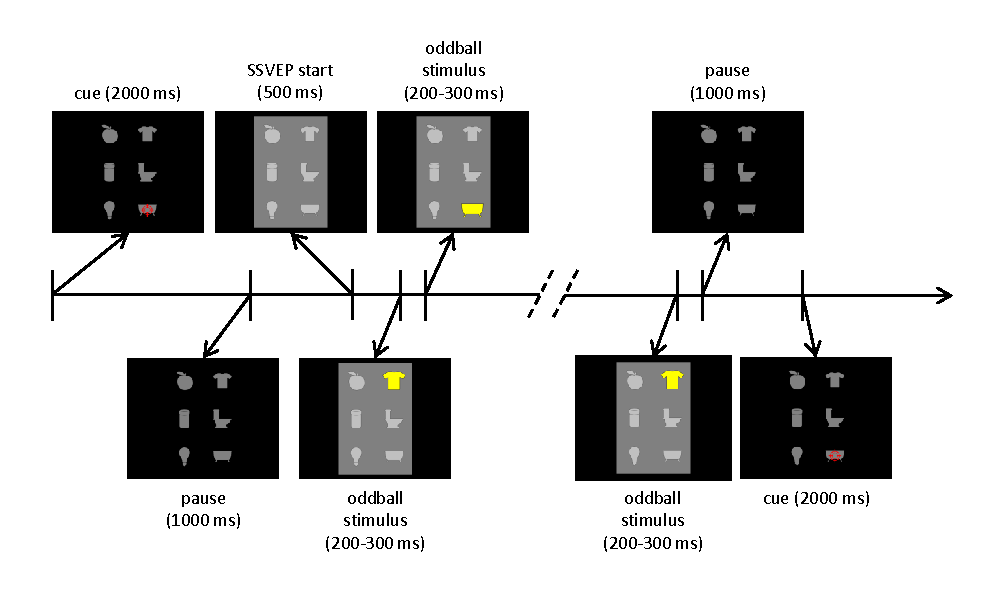
\includegraphics{pix/stimulationSequence}
\caption{stimulation sequence}
\label{fig:stimSeq}
\end{figure}

\begin{table*}[t]\scriptsize
\caption{
}
\label{table:TukeyTable}
\centering
\begin{tabular}{l r r l}
\toprule
Null hypothesis & Estimate & z value & p value \tabularnewline
\toprule
corr(h10/h12) - corr(h10/h08)  == 0 & $  0.003925 $ & $   0.628 $ & $ 0.99980 $\tabularnewline
corr(h10/h15) - corr(h10/h08)  == 0 & $ -0.011973 $ & $  -1.915 $ & $ 0.65869 $\tabularnewline
corr(h12/h08) - corr(h10/h08)  == 0 & $  0.004977 $ & $   0.796 $ & $ 0.99866 $\tabularnewline
corr(h12/h15) - corr(h10/h08)  == 0 & $  0.003652 $ & $   0.584 $ & $ 0.99989 $\tabularnewline
corr(h15/h08) - corr(h10/h08)  == 0 & $ -0.009712 $ & $  -1.553 $ & $ 0.87053 $\tabularnewline
corr(odd/h08) - corr(h10/h08)  == 0 & $ -0.105049 $ & $ -16.800 $ & $< 0.001 $\tabularnewline
corr(odd/h10) - corr(h10/h08)  == 0 & $ -0.124755 $ & $ -19.952 $ & $< 0.001 $\tabularnewline
corr(odd/h12) - corr(h10/h08)  == 0 & $ -0.100126 $ & $ -16.013 $ & $< 0.001 $\tabularnewline
corr(odd/h15) - corr(h10/h08)  == 0 & $ -0.084591 $ & $ -13.528 $ & $< 0.001 $\tabularnewline
corr(h10/h15) - corr(h10/h12)  == 0 & $ -0.015898 $ & $  -2.543 $ & $ 0.24549 $\tabularnewline
corr(h12/h08) - corr(h10/h12)  == 0 & $  0.001052 $ & $   0.168 $ & $ 1.00000 $\tabularnewline
corr(h12/h15) - corr(h10/h12)  == 0 & $ -0.000273 $ & $  -0.044 $ & $ 1.00000 $\tabularnewline
corr(h15/h08) - corr(h10/h12)  == 0 & $ -0.013637 $ & $  -2.181 $ & $ 0.46983 $\tabularnewline
corr(odd/h08) - corr(h10/h12)  == 0 & $ -0.108974 $ & $ -17.428 $ & $< 0.001 $\tabularnewline
corr(odd/h10) - corr(h10/h12)  == 0 & $ -0.128680 $ & $ -20.580 $ & $< 0.001 $\tabularnewline
corr(odd/h12) - corr(h10/h12)  == 0 & $ -0.104052 $ & $ -16.641 $ & $< 0.001 $\tabularnewline
corr(odd/h15) - corr(h10/h12)  == 0 & $ -0.088516 $ & $ -14.156 $ & $< 0.001 $\tabularnewline
corr(h12/h08) - corr(h10/h15)  == 0 & $  0.016950 $ & $   2.711 $ & $ 0.16923 $\tabularnewline
corr(h12/h15) - corr(h10/h15)  == 0 & $  0.015625 $ & $   2.499 $ & $ 0.26901 $\tabularnewline
corr(h15/h08) - corr(h10/h15)  == 0 & $  0.002261 $ & $   0.362 $ & $ 1.00000 $\tabularnewline
corr(odd/h08) - corr(h10/h15)  == 0 & $ -0.093076 $ & $ -14.885 $ & $< 0.001 $\tabularnewline
corr(odd/h10) - corr(h10/h15)  == 0 & $ -0.112782 $ & $ -18.037 $ & $< 0.001 $\tabularnewline
corr(odd/h12) - corr(h10/h15)  == 0 & $ -0.088153 $ & $ -14.098 $ & $< 0.001 $\tabularnewline
corr(odd/h15) - corr(h10/h15)  == 0 & $ -0.072618 $ & $ -11.614 $ & $< 0.001 $\tabularnewline
corr(h12/h15) - corr(h12/h08)  == 0 & $ -0.001325 $ & $  -0.212 $ & $ 1.00000 $\tabularnewline
corr(h15/h08) - corr(h12/h08)  == 0 & $ -0.014689 $ & $  -2.349 $ & $ 0.35712 $\tabularnewline
corr(odd/h08) - corr(h12/h08)  == 0 & $ -0.110026 $ & $ -17.596 $ & $< 0.001 $\tabularnewline
corr(odd/h10) - corr(h12/h08)  == 0 & $ -0.129732 $ & $ -20.748 $ & $< 0.001 $\tabularnewline
corr(odd/h12) - corr(h12/h08)  == 0 & $ -0.105104 $ & $ -16.809 $ & $< 0.001 $\tabularnewline
corr(odd/h15) - corr(h12/h08)  == 0 & $ -0.089568 $ & $ -14.324 $ & $< 0.001 $\tabularnewline
corr(h15/h08) - corr(h12/h15)  == 0 & $ -0.013364 $ & $  -2.137 $ & $ 0.50038 $\tabularnewline
corr(odd/h08) - corr(h12/h15)  == 0 & $ -0.108701 $ & $ -17.384 $ & $< 0.001 $\tabularnewline
corr(odd/h10) - corr(h12/h15)  == 0 & $ -0.128407 $ & $ -20.536 $ & $< 0.001 $\tabularnewline
corr(odd/h12) - corr(h12/h15)  == 0 & $ -0.103779 $ & $ -16.597 $ & $< 0.001 $\tabularnewline
corr(odd/h15) - corr(h12/h15)  == 0 & $ -0.088243 $ & $ -14.112 $ & $< 0.001 $\tabularnewline
corr(odd/h08) - corr(h15/h08)  == 0 & $ -0.095337 $ & $ -15.247 $ & $< 0.001 $\tabularnewline
corr(odd/h10) - corr(h15/h08)  == 0 & $ -0.115043 $ & $ -18.399 $ & $< 0.001 $\tabularnewline
corr(odd/h12) - corr(h15/h08)  == 0 & $ -0.090415 $ & $ -14.460 $ & $< 0.001 $\tabularnewline
corr(odd/h15) - corr(h15/h08)  == 0 & $ -0.074879 $ & $ -11.975 $ & $< 0.001 $\tabularnewline
corr(odd/h10) - corr(odd/h08)  == 0 & $ -0.019706 $ & $  -3.152 $ & $ 0.05210 $\tabularnewline
corr(odd/h12) - corr(odd/h08)  == 0 & $  0.004923 $ & $   0.787 $ & $ 0.99877 $\tabularnewline
corr(odd/h15) - corr(odd/h08)  == 0 & $  0.020458 $ & $   3.272 $ & $ 0.03590 $\tabularnewline
corr(odd/h12) - corr(odd/h10)  == 0 & $  0.024629 $ & $   3.939 $ & $ 0.00359 $\tabularnewline
corr(odd/h15) - corr(odd/h10)  == 0 & $  0.040164 $ & $   6.423 $ & $< 0.001 $\tabularnewline
corr(odd/h15) - corr(odd/h12)  == 0 & $  0.015536 $ & $   2.485 $ & $ 0.27654 $\tabularnewline
\bottomrule
\end{tabular}
\end{table*}

%===================================================================================================================
%                                             TABLES
%===================================================================================================================


%===================================================================================================================
%                                             FIGURES
%===================================================================================================================
\clearpage

%-------------------------------------------------------------------------------------------------------------------
% oddball pix
%-------------------------------------------------------------------------------------------------------------------
\begin{figure}[t]
\centering
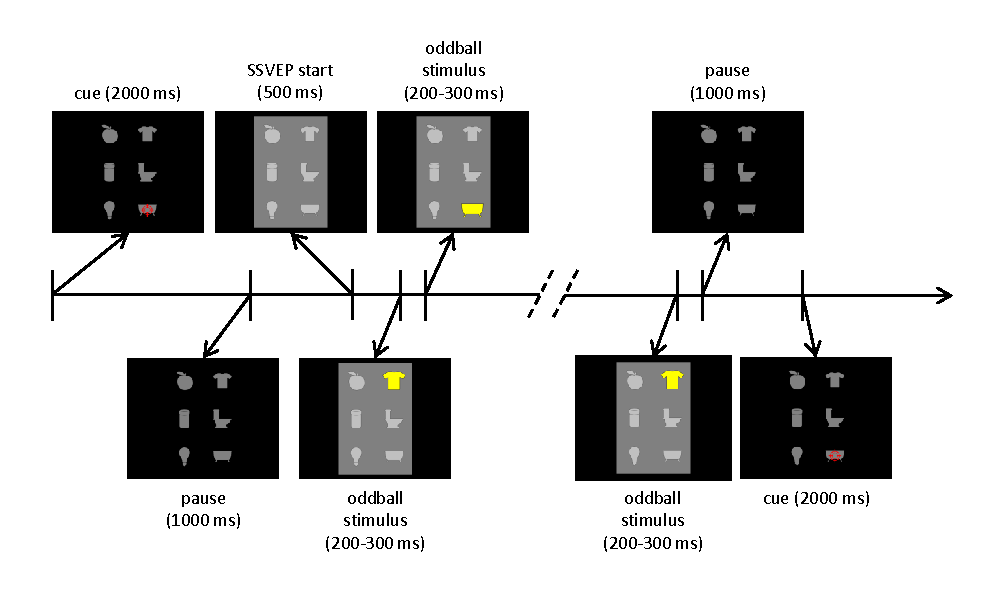
\includegraphics{pix/stimulationSequence}
\caption{stimulation sequence}
\label{fig:stimSeq}
\end{figure}

%\section{Acronyms}
%\begin{acronym}
%    \acro{SSVEP}{Steady-State Visually Evoked Potential}
%\end{acronym}

\end{document}
